\section{Service-Oriented Architecture (SOA)}
\subsection{Proceso de Análisis y diseño orientados a servicios}

En la etapa de análisis y diseño, el arquitecto de software se reúne con un analista de negocio, el cual diseñará unos servicios candidatos que después se convertirán en los servicios incluidos en los blueprints. Luego de tener los planos, el arquitecto escoge un subconjunto de dichos candidatos a servicios para ser implementados físicamente, dotándolos de algún método para realizar la composición de servicios. En la figura \ref{fig:seis} se muestra el proceso de análisis y diseño orientado a servicios.

\begin{figure}[!htb]
  \begin{center}
    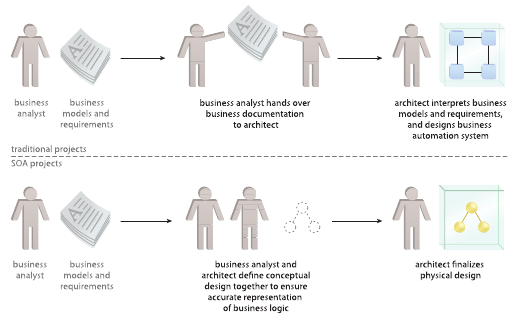
\includegraphics[width=11cm]{./imagenes/6.png}
    \caption{proceso de análisis y diseño orientado a servicios}
    \label{fig:seis}
    \textbf{Fuente:}  \cite{soa_principles}
  \end{center}
\end{figure}

\subsection{Metas y beneficios de la computación orientada a servicios }

Las metas y los beneficios que trae la implementación de la computación orientada a servicios en una organización son:

\begin{itemize}
  \item \textbf{Incremento de la interoperabilidad intrínseca}: Es una meta de la computación orientada a servicios ya que la composición de servicios requiere que, sin necesidad de integrar un servicio con el otro, estos puedan intercambiar información para desarrollar la funcionalidad a la que han sido inscritos. Aplicando principios de diseño orientados a servicios, así como también estándares de diseño orientados a servicios, se logra el incremento de la interoperabilidad intrínseca.
  \item \textbf{Federación incrementada}: Un entorno de TI federado es aquel en el cual los recursos y aplicaciones se manejan y gobiernan con autonomía y por sí mismos. En el ámbito de la orientación a servicios, cada servicio puede tener su propia implementación independiente y aun así comunicarse. Esto se logra por medio de una especial atención a los estándares de diseño.
  \item \textbf{Incremento de opciones en la escogencia de proveedores de servicios}: Como la federación en la computación orientada a servicios es una meta, la escogencia de proveedores de servicios diferentes es un beneficio ya que la composición de servicios puede ser lograda sin importar que proveedor provea de un servicio específico.
  \item \textbf{Incremento de la alineación entre el negocio y las tecnologías}: Ya que en el proceso de diseño actúan tanto el analista de negocio como el arquitecto de software, la alineación entre negocio y tecnologías es incrementada. La reconfiguración en la composición de servicios, además, provee alineación extra al poder cambiar el proceso de negocio y la composición de los servicios al mismo tiempo.
  \item \textbf{ROI}: Al hacerse inventarios de servicios y, además, ser los servicios reutilizables a lo largo del tiempo y compuestos de diferente forma gracias a la composición de servicios, se da una relación costo/beneficio más baja que con otros paradigmas usados.
  \item \textbf{Agilidad organizacional incrementada}: Debido a la orientación a servicios, se hace una composición rápida de los servicios que se tengan y se crean los que se necesiten para agilizar el proceso del departamento de TI y así agilizar los procesos subyacentes.
  \item \textbf{Reducción de cargas al departamento TI}: Debido a la agilidad organizacional cuando es aplicada la orientación a servicios, son reducidos costos operacionales (tiempo u otros recursos) y el departamento de TI adquiere un papel activo en el sector estratégico.
\end{itemize}
